\documentclass{article}
\usepackage{graphicx} 
\usepackage{amsmath}
\usepackage{hyperref}
\usepackage[table, dvipsnames, xcdraw]{xcolor}
\usepackage{array}
\usepackage{makecell}
\usepackage{cite}
\usepackage[left=1in, right=1in, top=1in, bottom=1in]{geometry}

\graphicspath{{../figures}}

\title{Design of Rotorcraft}
\author{Brighton Smith}

\begin{document}

\maketitle

\section{Introduction}
In this report, I walk through the primary considerations that need to be made for the design of our rotorcraft. I use a number of methods ranging from mathematical theory to empirical test data to risk assessment. This report is meant to give our stakeholders a comprehensive understanding of our current status as well as some suggestions to move forward. 

In Sec. \ref{sec:num_props}, I start with an assessment of the ideal number of propellers for our rotorcraft given our design requirements and readily available parts. In Sec. \ref{sec:motor-props}, I move to examining the best motor-propeller combination for our system using physics, test data, and risk analysis. I summarize the findings of this report in Sec. \ref{sec:conclusion}, and provide an alternative method of flight that is thrifty and guarantees flight (though it directly contradicts a requirement) in Sec. \ref{sec:appendix}. Since this report is quite exhaustive, I would recommend prioritizing reading Secs. \ref{sec:risk}, \ref{sec:conclusion}, and \ref{sec:appendix}. 

\section{Number of Propellers}\label{sec:num_props}
The initial factor to be considered in the design of our rotorcraft is the number of propellers. Six propellers (hexacopter) was the initial suggestion, but upon formalized analysis, it was found that an eight propeller rotorcraft (octocopter) may be the optimal configuration. The relevant mathematical framework that yields this conclusion is blade element theory \cite{GUDMUNDSSON2014581}, which produces the following governing equations:
\begin{equation}
    T \propto \rho n^2 D^4
\end{equation}
\begin{equation}\label{eq:P}
    P \propto \rho n^3 D^5
\end{equation}
\begin{equation}\label{eq:F_d}
    F_d \propto V^2 = (\pi nD)^2
\end{equation}
where $T$ is the thrust produced by a propeller of diameter $D$ and rotating at speed $n$, $\rho$ is the air density, $P$ is the power required by the same propeller to achieve hover, $F_d$ is the drag force experienced by the propeller, and $V$ is the blade velocity. To use these equations in our context, consider two propellers producing the same thrust $T$, with diameters $D_1$ and $D_2$ and rotating at $n_1$ and $n_2$, respectively. Then we have
\begin{equation}
    T \propto \rho n_1^2 D_1^4 = \rho n_2^2 D_2^4,
\end{equation}
and simplifying gives
\begin{equation}\label{eq:n-relation}
    n_2 = n_1(\frac{D_1}{D_2})^2.
\end{equation}
If $D_1 < D_2$, then $n_2 < n_1$, meaning the larger propeller can produce the same thrust at a lower rotational speed. Substitution of Eq. \ref{eq:n-relation} into Eq. \ref{eq:F_d} gives
\begin{equation}
    \frac{F_{d,2}}{F_{d,1}} = (\frac{D_1}{D_2})^2,
\end{equation}
meaning that $F_{d,2} << F_{d,1}$ for $D_1 < D_2$. This indicates that drag is more heavily affected by the rotation of the blades than propeller diameter. In other words, it is optimal to increase the size of the blades and work at a lower RPM to achieve a thrust requirement than to decrease the blade size and increase the RPM. Therefore, an octocopter can mitigate drag force purely by increasing the \textit{effective swept area} of the propellers as opposed to a hexacopter. When fixing propeller size, as is done here, adding propellers should always make the system more efficient.

However, while the math does hold true, Figs. \ref{fig:uav_comparison} and \ref{fig:uav_difference_comparison} indicate that the difference is marginal at best, given our current motor-propeller pairing. Notice from Fig. \ref{fig:uav_difference_comparison} that at our maximum theoretical engine output, the additional thrust of an octocopter is about 2 lbs. From Tab. \ref{tab:powertrain_weight}, it can be observed that the added powertrain weight of an octocopter is nearly 2 lbs, which outweighs the thrust gain below approximately 90\% efficient engine output (which is itself unrealistic).\footnote{Note that in this document, the powertrain weight is defined as the cumulative sum of the propellers, motors, and electronic speed controllers.} Therefore, it is made clear that \textbf{a hexacopter configuration is optimal for our design.}

\begin{figure}[htbp]
    \centering
    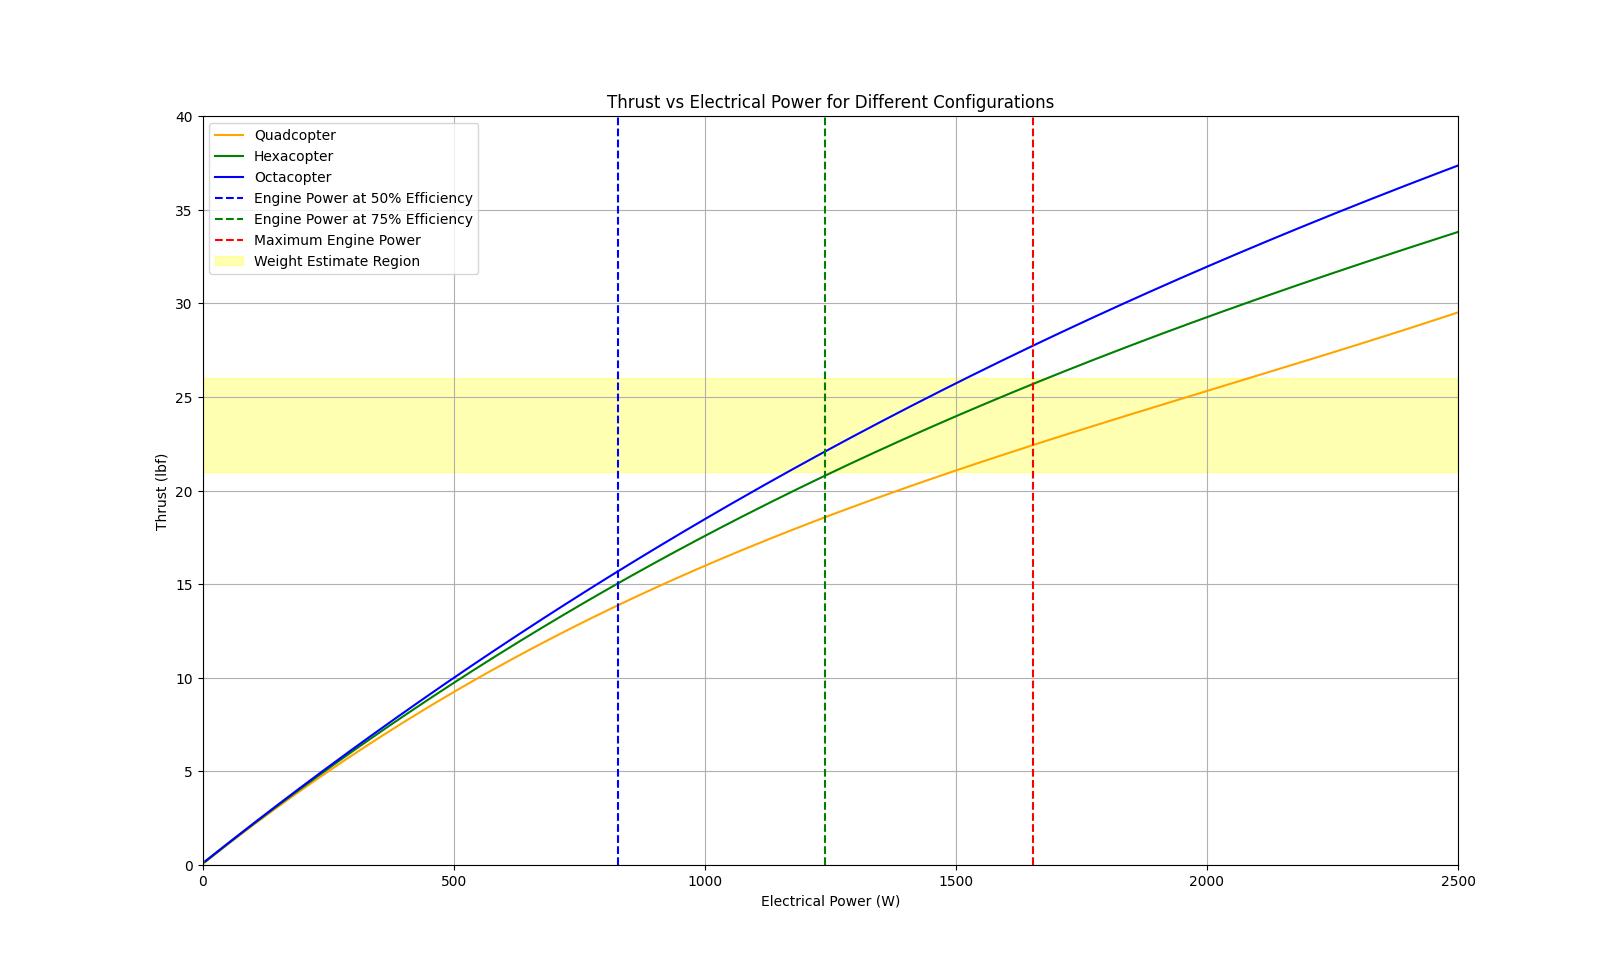
\includegraphics[width=0.8\textwidth]{UAV Comparison (experimental).png}
    \caption{A comparison of thrust and power input for different propeller counts, considering our current motor-propeller pairing.}
    \label{fig:uav_comparison}
\end{figure}
\begin{figure}[htbp]
    \centering
    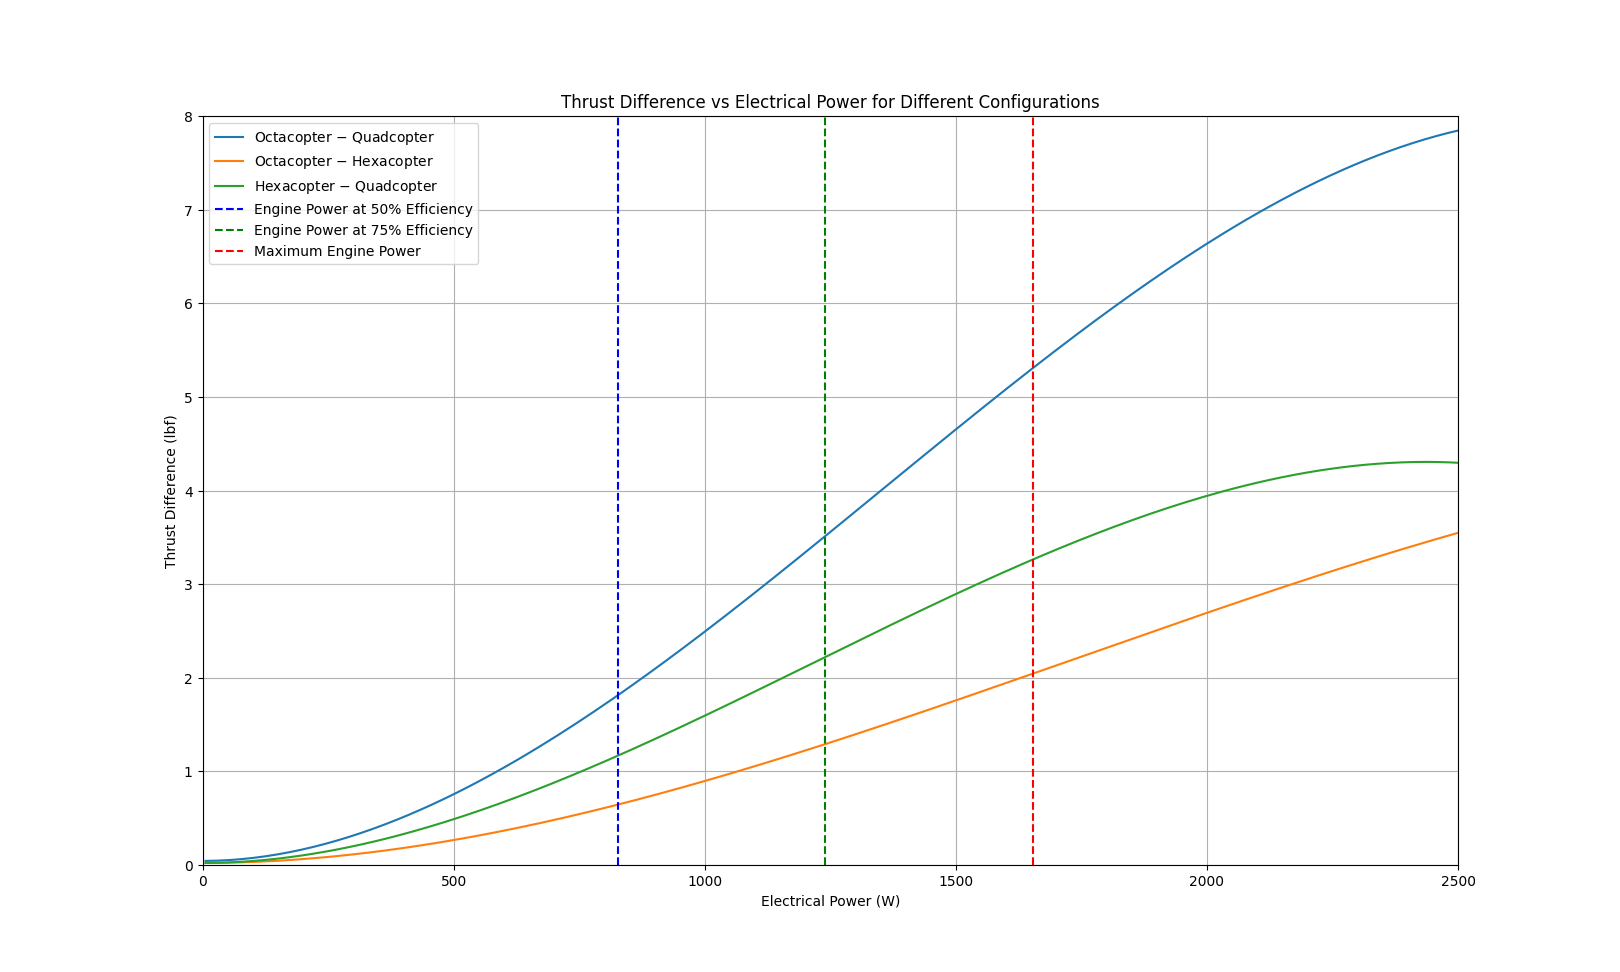
\includegraphics[width=0.8\textwidth]{UAV Difference Comparison (experimental).png}
    \caption{A comparison of \textit{total} thrust difference and power input for different propeller counts, considering our current motor-propeller pairing.}
    \label{fig:uav_difference_comparison}
\end{figure}

\begin{table}[h]
    \centering
    \begin{tabular}{|c|c|c|}
        \hline
        \rowcolor{lightgray} % Header row color
        \textbf{Hexacopter Powertrain Weight (lbs)} & \textbf{Octacopter Powertrain Weight (lbs)} & \textbf{Weight Difference} \\
        \hline
        5.323 & 7.100 & 1.777 \\
        \hline
    \end{tabular}
    \caption{Powertrain weight comparison for our current motor-propeller pairing.}
    \label{tab:powertrain_weight}
\end{table}

\section{Motor-Propeller Pairing Selection}\label{sec:motor-props}
Now that the configuration has been established, it is important to choose a motor-propeller pairing that \textit{minimizes the electrical power input in our weight estimate region}. Now that we hold the number of propellers constant, it must be realized that there are only two ways to increase thrust output: (1) increasing the total swept area of the blades while keeping RPM constant, or (2) increasing the RPM while keeping the total swept area constant. From the equations developed in Sec. \ref{sec:num_props}, it was shown that larger propellers spinning slowly are better at reducing drag than smaller propellers spinning fast. This fact can be extended to the power domain as well. Substitution from Eq. \ref{eq:n-relation} into Eq. \ref{eq:P} gives
\begin{equation}
    P_2 \propto \rho n_1^3 \frac{D_1^6}{D_2},
\end{equation} 
and thus comparing $P_1$ and $P_2$ yields
\begin{equation}
    \frac{P_2}{P_1} = \frac{D_1}{D_2},
\end{equation}
indicating that $P_2 < P_1$ for $D_1 < D_2$. \textit{This means that a large propeller can generate the same amount of thrust at a lower power input than a small propeller.}

This principle is also empirically verified by the propeller efficiency curve plotted in Fig. \ref{fig:prop_efficiency}. Two observations can be made from the plot:
\begin{itemize}
    \item Propellers are higher functioning at lower RPM, meaning it is more desirable to increase the total swept area of the blades to increase thrust.
    \item Our current propellers are most efficient in the 2000-3000 RPM range, but we are expecting to operate in the 5000 RPM range, which means a dramatic efficiency reduction.
\end{itemize}

\begin{figure}[htbp]
    \centering
    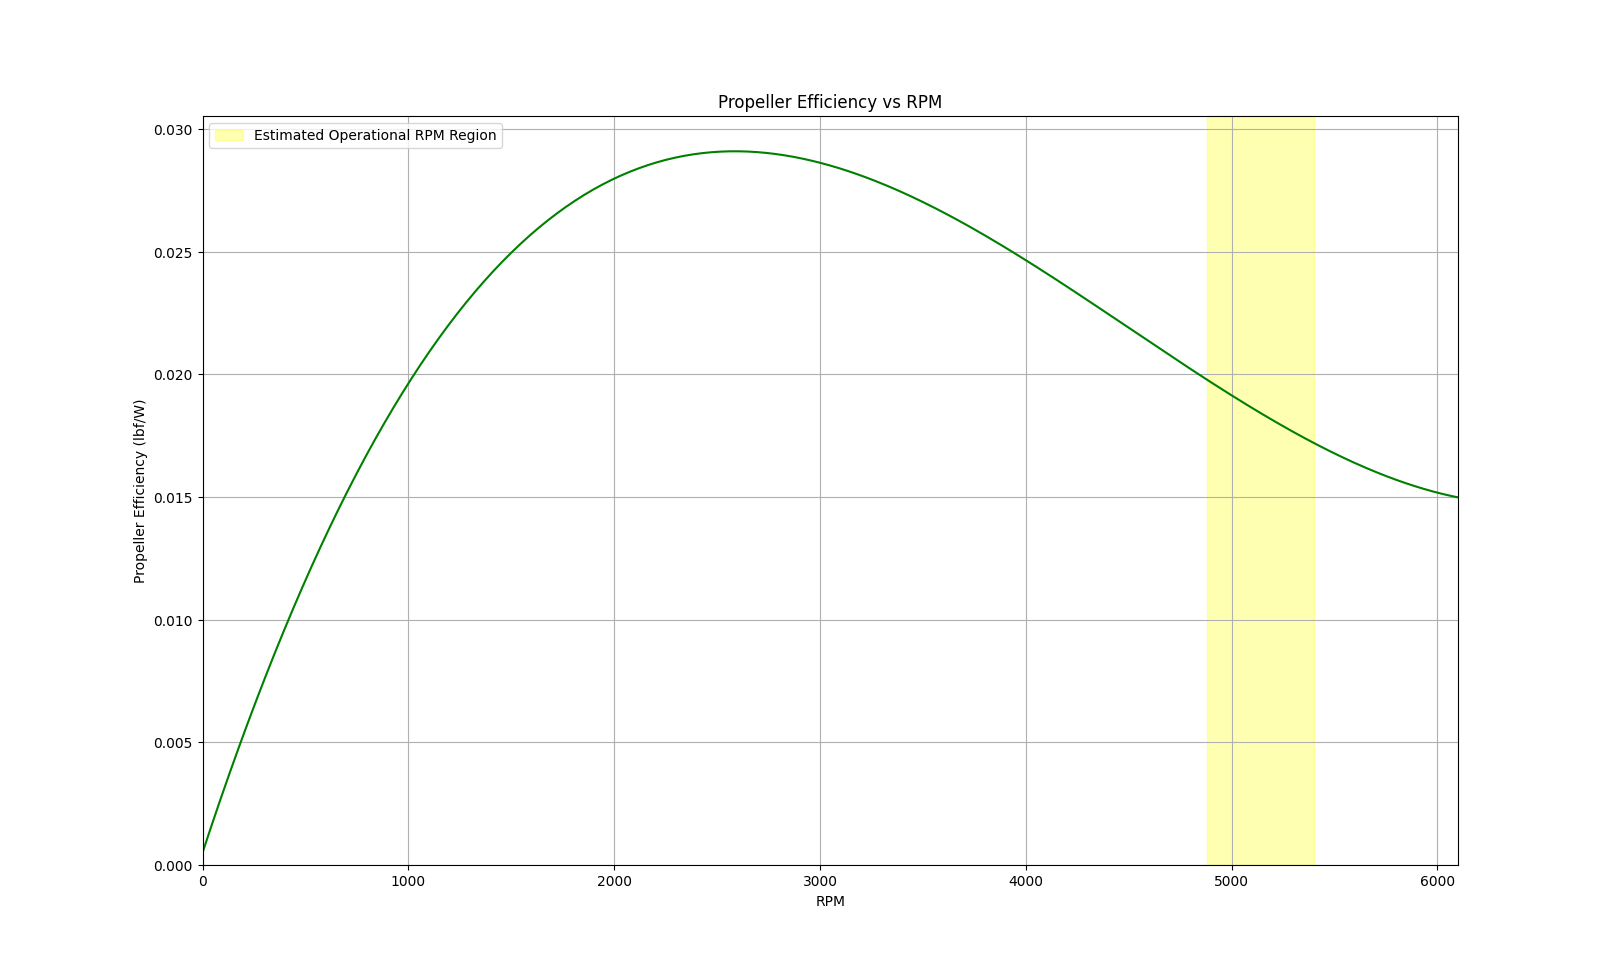
\includegraphics[width=0.8\textwidth]{Prop Efficiency vs RPM (experimental).png}
    \caption{A comparison of propeller efficiency and rotational speed using our Waco data.}
    \label{fig:prop_efficiency}
\end{figure}

The validity of these two points provides motivation to examine other motor-propeller pairings given our design requirements, even though we already have a set of both motors and propellers. There are two different options to be evaluated: (1) buying larger propellers only or, (2) buying new motors and propellers. 

\subsection{New Propellers Only}
Buying larger propellers only is certainly the most cost sensitive option since propellers are much less expensive than motors. Additionally, while larger propellers require more torque to be able to spin, they also can produce the same thrust as a smaller propeller at a lower RPM. This is desirable given the principle from blade element theory discussed earlier that propellers are generally more efficient at lower rotational speed. 

A demonstration of the effects of using new propellers with our current motors on the necessary power input can be seen in Figs. \ref{fig:prop_comparison_kv490} and \ref{fig:prop_difference_comparison_kv490}. Note that while the 16 in. and 18 in. propeller curves in the aforementioned figures were generated from experimental test data, the 20 in. propeller curve was made using Newton's polynomial coefficient interpolation method \cite{python}, since test data of the 20 in. propellers with our motors was not readily available. Therefore, the latter curve most likely strays from reality at high power input values. However, considering that \textbf{our engine only reached ~85\% the nominal maximum power output under the loading of a simple propeller}, it is reasonable to believe this curve gives an accurate portrayal of the added thrust benefit of 20 in. propellers for our working power region.

\begin{figure}[htbp]
    \centering
    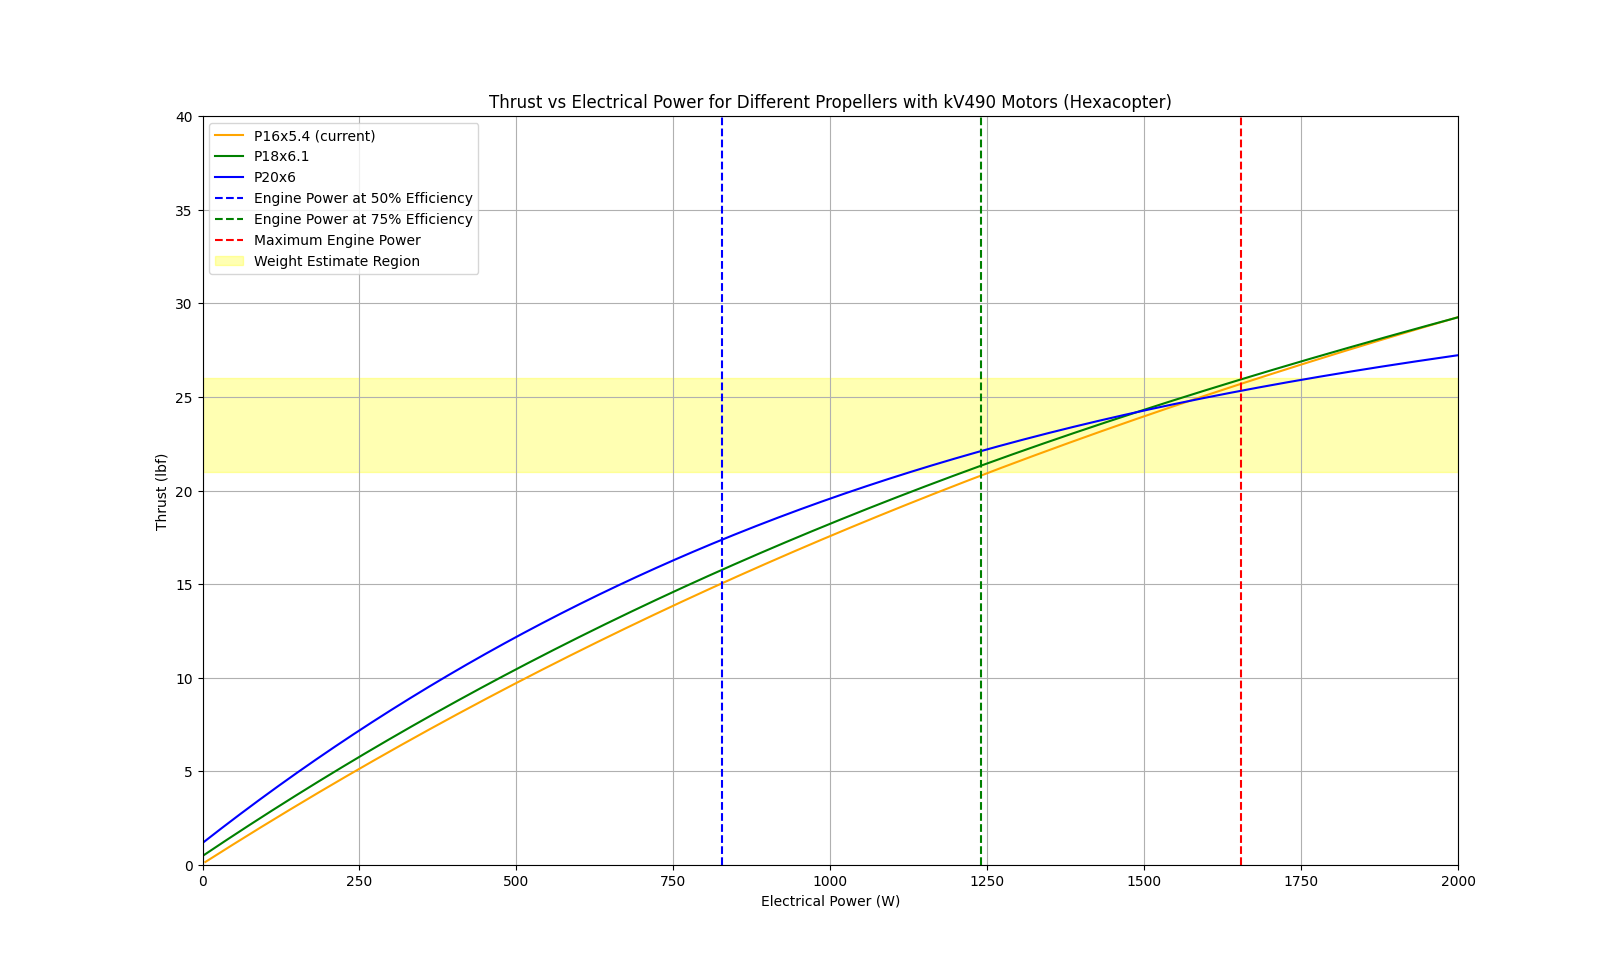
\includegraphics[width=0.8\textwidth]{Prop Comparison (kV490).png}
    \caption{A comparison of thrust and power input for different propellers using our current motors.}
    \label{fig:prop_comparison_kv490}
\end{figure}
\begin{figure}[htbp]
    \centering
    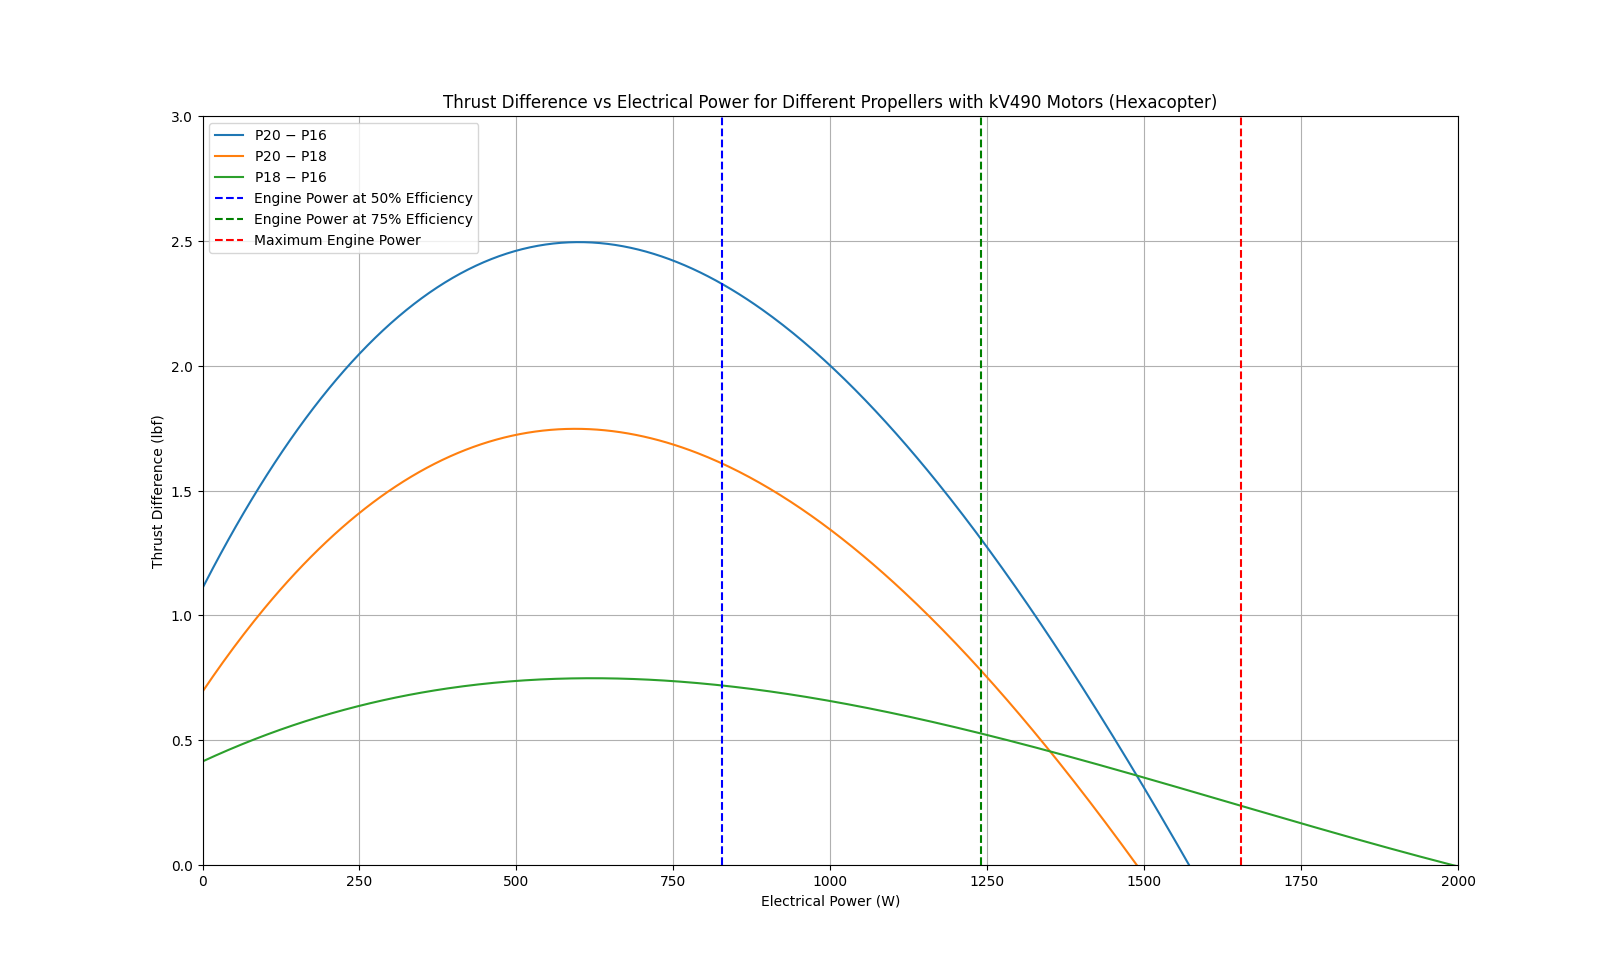
\includegraphics[width=0.8\textwidth]{Prop Difference Comparison (kV490).png}
    \caption{A comparison of \textit{total} thrust difference and power input for different propellers using our current motors.}
    \label{fig:prop_difference_comparison_kv490}
\end{figure}

By observing Fig. \ref{fig:prop_difference_comparison_kv490}, it can be seen that our motors are not expected to work efficiently with larger propellers. At 75\% engine efficiency, 20 in. propellers narrowly outperform our 16 in. propellers. Even less desirable is that the additional thrust benefit of 20 in. propellers monotonically decreases past $\sim$40\% engine efficiency. However, as evidenced by Tab. \ref{tab:prop_comparison}, the weight addition and cost of larger propellers is small.

\begin{table}[h]
    \centering
    \begin{tabular}{|c|c|c|c|}
        \hline
        \rowcolor{lightgray} % Header row color
         & \textbf{16 in. Props} & \textbf{18 in. Props} & \textbf{20 in. Props} \\
        \hline
        Powertrain Weight (lbs) & 5.323 & 5.408 & 5.616 \\
        \hline
        Total Cost (\$) & 188.70 & 248.70 & 326.70 \\
        \hline
    \end{tabular}
    \caption{Cost and weight comparison for different propellers given a hexacopter configuration and using our current motors.}
    \label{tab:prop_comparison}
\end{table}

\subsection{New Motors and Propellers}\label{sec:new-motors-props}
The other option to review is larger propellers paired with different motors. While the added cost of motors is significant, Figs. \ref{fig:prop_comparison_experimental} and \ref{fig:prop_difference_comparison_experimental} demonstrate that the additional thrust is also significant. Notice in Fig. \ref{fig:prop_comparison_experimental} that at 75\% engine efficiency, the 20 in. propeller curve is entirely above our weight estimate region, while the 16 in. propeller curve is below it. Additionally, observe from Fig. \ref{fig:prop_difference_comparison_experimental} that the total thrust difference between the 20 in. propellers with Kv230 motors and our current 16 in. propellers with Kv490 motors is $\sim$5 lbf at 50\% engine efficiency, and $\sim$6.5 lbf at maximum theoretical engine output. Even more notable is the monotonically increasing behavior of the difference curve in the same plot, meaning as our engine is more efficient, we can expect a better thrust benefit (contrast with Fig. \ref{fig:prop_difference_comparison_kv490} for instance).

\begin{figure}[htbp]
    \centering
    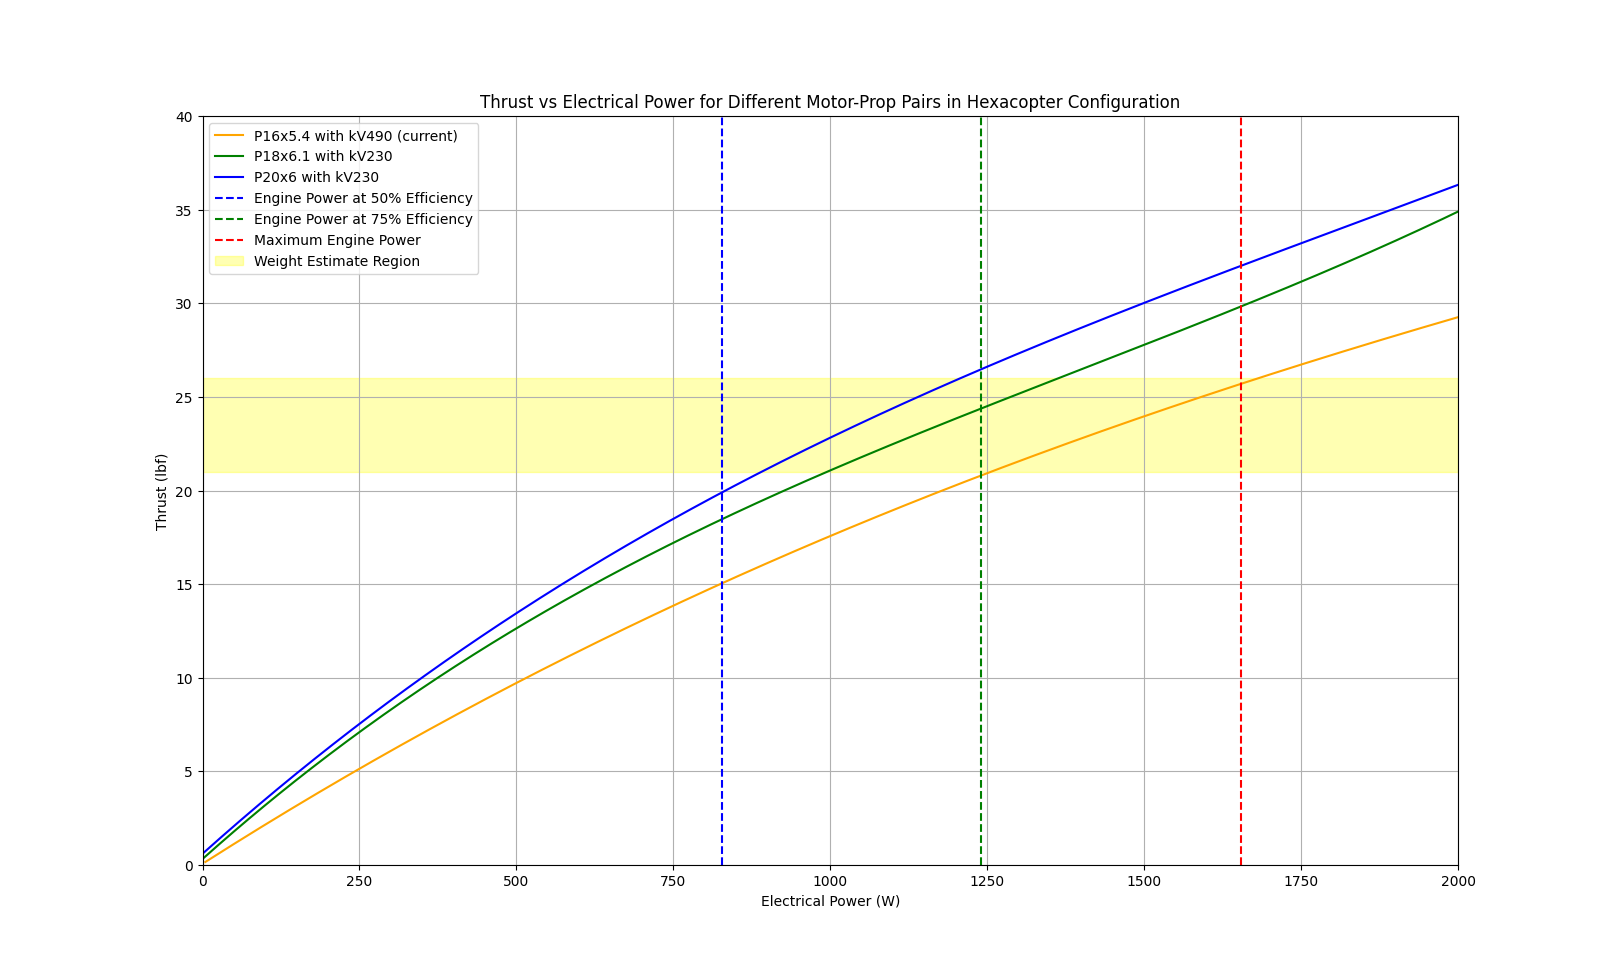
\includegraphics[width=0.8\textwidth]{Prop Comparison (experimental).png}
    \caption{A comparison of thrust and power input for different propellers and different motors.}
    \label{fig:prop_comparison_experimental}
\end{figure}
\begin{figure}[htbp]
    \centering
    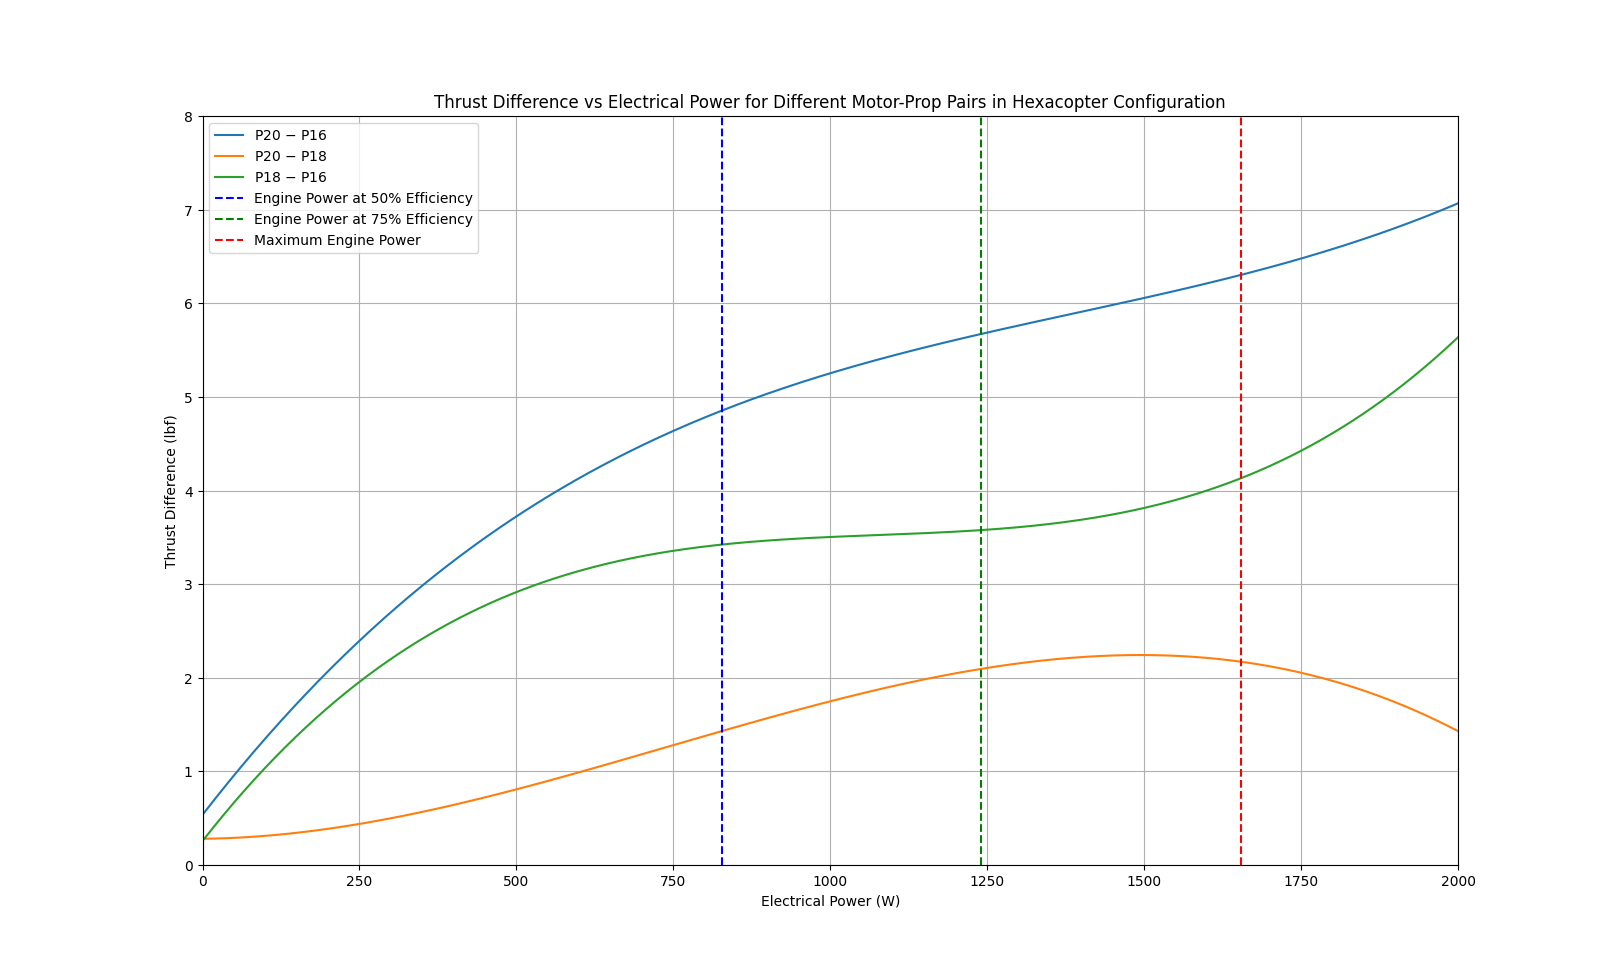
\includegraphics[width=0.8\textwidth]{Prop Difference Comparison (experimental).png}
    \caption{A comparison of \textit{total} thrust difference and power input for different propellers and different motors.}
    \label{fig:prop_difference_comparison_experimental}
\end{figure}

Because of the significant thrust benefit of the newly suggested propellers and motors, one might expect that the weight increase would also be significant, thus canceling each other out. However, as seen in Tab. \ref{tab:motor_prop_comparison}, the opposite is actually true, and the powertrain weight of the 20 in. propellers with Kv230 motors is \textit{lighter} than our current powertrain weight by almost 1.5 lbs. The only additional weight consideration we would need to account for is the larger airframe required for 20 in. propellers. From Tab. \ref{tab:motor_prop_comparison}, one can see that the major downside is the additional cost required. In order to better quantify the pros and cons of upgrading to the new system, a risk assessment has been provided in the subsequent section. 

\begin{table}[h]
    \centering
    \begin{tabular}{|c|c|c|c|}
        \hline
        \rowcolor{lightgray} % Header row color
        & \makecell{\textbf{16 in. Props} \\ \textbf{x Kv490 Motors}} & \makecell{\textbf{18 in. Props} \\ \textbf{x Kv230 Motors}} & \makecell{\textbf{20 in. Props} \\ \textbf{x Kv230 Motors}} \\
        \hline
        \textbf{Powertrain Weight (lbs)} & 5.323 & 3.938 & 4.054 \\
        \hline
        \textbf{Total Cost (\$)} & 1088.10 & 1568.64 & 1646.64 \\
        \hline
    \end{tabular}
    \caption{Cost and weight comparison for different motor-propeller pairs given a hexacopter configuration.}
    \label{tab:motor_prop_comparison}
\end{table}

\subsection{Risk Assessment}\label{sec:risk}
One way to evaluate the performance of the motor-propeller pairings put forth in Sec. \ref{sec:new-motors-props} is to look at the feasibility to hover---one of our major requirements---given a system weight and efficiency.\footnote{Requirement 9: The system shall be capable of hovering for 20 min. (T), 1 hr (O).} A matrix such as this has been provided for each solicited pairing in Tabs. \ref{tab:hover_likelihood_matrix_16}-\ref{tab:hover_likelihood_matrix_20} along with an interpretive key in Tab. \ref{tab:key_likelihood_matrix}. Note that in each matrix, the weight range is 21-26 lbs, since this is our estimated weight region. Additionally, the system efficiency metric is based on the amount of electrical power that reaches the powertrain from the engine. \textbf{It is imperative to note that the system efficiency only considers the engine, meaning that these matrices are for a system capable of sustainable flight (i.e. charging the battery during flight, which is another one of our requirements).}\footnote{Requirement 4: The engine shall drive the on-board alternator, which will charge the storage battery via a battery management system.} If draining the battery continuously for the duration of the flight is allowable, then Tabs. \ref{tab:hover_likelihood_matrix_16}-\ref{tab:hover_likelihood_matrix_20} would look (somewhat) different. A theoretical exploration of time of flight variation for the continuously draining battery case has been included in Sec. \ref{sec:appendix}, but since it is theoretical and directly goes against a requirement, it was not included in the primary risk assessment.

The following process was used in the creation of Tabs. \ref{tab:hover_likelihood_matrix_16}-\ref{tab:hover_likelihood_matrix_20}:
\begin{enumerate}
    \item Determine the estimated weight region for our system given our current weight roll-up.
    \item Determine the power value corresponding to the system efficiency (based on the manufacturer specified maximum engine output power).
    \item Use empirical motor-propeller data to interpolate the thrust value corresponding to the power value calculated in step 2.
    \item Calculate the percent difference between the thrust value determined in step 3 and the weight specification in step 1.
    \item Create a key that maps the percent difference to a hover likelihood metric (Tab. \ref{tab:key_likelihood_matrix}).
\end{enumerate}

\begin{table}[h]
    \centering
    \begin{tabular}{|c|c|c|c|c|c|c|c|}
        \hline
 & 40\% & 50\% & 60\% & 70\% & 80\% & 90\% & 100\%  \\
        \hline
        21 lbs & \cellcolor{red!80} Very Low & \cellcolor{red!80} Very Low & \cellcolor{red!80} Very Low & \cellcolor{red!20} Low & \cellcolor{yellow!60} Medium & \cellcolor{ForestGreen!80} Very High & \cellcolor{ForestGreen!80} Very High \\
        \hline
        22 lbs & \cellcolor{red!80} Very Low & \cellcolor{red!80} Very Low & \cellcolor{red!80} Very Low & \cellcolor{red!80} Very Low & \cellcolor{yellow!60} Medium & \cellcolor{ForestGreen!40} High & \cellcolor{ForestGreen!80} Very High \\
        \hline
        23 lbs & \cellcolor{red!80} Very Low & \cellcolor{red!80} Very Low & \cellcolor{red!80} Very Low & \cellcolor{red!80} Very Low & \cellcolor{red!20} Low & \cellcolor{yellow!60} Medium & \cellcolor{ForestGreen!80} Very High \\
        \hline
        24 lbs & \cellcolor{red!80} Very Low & \cellcolor{red!80} Very Low & \cellcolor{red!80} Very Low & \cellcolor{red!80} Very Low & \cellcolor{red!20} Low & \cellcolor{yellow!60} Medium & \cellcolor{ForestGreen!40} High \\
        \hline
        25 lbs & \cellcolor{red!80} Very Low & \cellcolor{red!80} Very Low & \cellcolor{red!80} Very Low & \cellcolor{red!80} Very Low & \cellcolor{red!80} Very Low & \cellcolor{red!20} Low & \cellcolor{yellow!60} Medium \\
        \hline
        26 lbs & \cellcolor{red!80} Very Low & \cellcolor{red!80} Very Low & \cellcolor{red!80} Very Low & \cellcolor{red!80} Very Low & \cellcolor{red!80} Very Low & \cellcolor{red!80} Very Low & \cellcolor{yellow!60} Medium \\
        \hline
    \end{tabular}
    \caption{Hover flight likelihood matrix for 16 in. propellers with Kv490 motors (current).}
    \label{tab:hover_likelihood_matrix_16}
\end{table}

\begin{table}[h]
    \centering
    \begin{tabular}{|c|c|c|c|c|c|c|c|}
        \hline
 & 40\% & 50\% & 60\% & 70\% & 80\% & 90\% & 100\%  \\
        \hline
        21 lbs & \cellcolor{red!80} Very Low & \cellcolor{red!80} Very Low & \cellcolor{yellow!60} Medium & \cellcolor{ForestGreen!80} Very High & \cellcolor{ForestGreen!80} Very High & \cellcolor{ForestGreen!80} Very High & \cellcolor{ForestGreen!80} Very High \\
        \hline
        22 lbs & \cellcolor{red!80} Very Low & \cellcolor{red!80} Very Low & \cellcolor{red!20} Low & \cellcolor{ForestGreen!40} High & \cellcolor{ForestGreen!80} Very High & \cellcolor{ForestGreen!80} Very High & \cellcolor{ForestGreen!80} Very High \\
        \hline
        23 lbs & \cellcolor{red!80} Very Low & \cellcolor{red!80} Very Low & \cellcolor{red!20} Low & \cellcolor{yellow!60} Medium & \cellcolor{ForestGreen!80} Very High & \cellcolor{ForestGreen!80} Very High & \cellcolor{ForestGreen!80} Very High \\
        \hline
        24 lbs & \cellcolor{red!80} Very Low & \cellcolor{red!80} Very Low & \cellcolor{red!80} Very Low & \cellcolor{yellow!60} Medium & \cellcolor{ForestGreen!40} High & \cellcolor{ForestGreen!80} Very High & \cellcolor{ForestGreen!80} Very High \\
        \hline
        25 lbs & \cellcolor{red!80} Very Low & \cellcolor{red!80} Very Low & \cellcolor{red!80} Very Low & \cellcolor{red!20} Low & \cellcolor{yellow!60} Medium & \cellcolor{ForestGreen!80} Very High & \cellcolor{ForestGreen!80} Very High \\
        \hline
        26 lbs & \cellcolor{red!80} Very Low & \cellcolor{red!80} Very Low & \cellcolor{red!80} Very Low & \cellcolor{red!80} Very Low & \cellcolor{yellow!60} Medium & \cellcolor{ForestGreen!40} High & \cellcolor{ForestGreen!80} Very High \\
        \hline
    \end{tabular}
    \caption{Hover flight likelihood matrix for 18 in. propellers with Kv230 motors.}
    \label{tab:hover_likelihood_matrix_18}
\end{table}

\begin{table}[h]
    \centering
    \begin{tabular}{|c|c|c|c|c|c|c|c|}
        \hline
 & 40\% & 50\% & 60\% & 70\% & 80\% & 90\% & 100\%  \\
        \hline
        21 lbs & \cellcolor{red!80} Very Low & \cellcolor{red!20} Low & \cellcolor{ForestGreen!40} High & \cellcolor{ForestGreen!80} Very High & \cellcolor{ForestGreen!80} Very High & \cellcolor{ForestGreen!80} Very High & \cellcolor{ForestGreen!80} Very High \\
        \hline
        22 lbs & \cellcolor{red!80} Very Low & \cellcolor{red!80} Very Low & \cellcolor{yellow!60} Medium & \cellcolor{ForestGreen!80} Very High & \cellcolor{ForestGreen!80} Very High & \cellcolor{ForestGreen!80} Very High & \cellcolor{ForestGreen!80} Very High \\
        \hline
        23 lbs & \cellcolor{red!80} Very Low & \cellcolor{red!80} Very Low & \cellcolor{yellow!60} Medium & \cellcolor{ForestGreen!40} High & \cellcolor{ForestGreen!80} Very High & \cellcolor{ForestGreen!80} Very High & \cellcolor{ForestGreen!80} Very High \\
        \hline
        24 lbs & \cellcolor{red!80} Very Low & \cellcolor{red!80} Very Low & \cellcolor{red!20} Low & \cellcolor{yellow!60} Medium & \cellcolor{ForestGreen!80} Very High & \cellcolor{ForestGreen!80} Very High & \cellcolor{ForestGreen!80} Very High \\
        \hline
        25 lbs & \cellcolor{red!80} Very Low & \cellcolor{red!80} Very Low & \cellcolor{red!80} Very Low & \cellcolor{yellow!60} Medium & \cellcolor{ForestGreen!40} High & \cellcolor{ForestGreen!80} Very High & \cellcolor{ForestGreen!80} Very High \\
        \hline
        26 lbs & \cellcolor{red!80} Very Low & \cellcolor{red!80} Very Low & \cellcolor{red!80} Very Low & \cellcolor{yellow!60} Medium & \cellcolor{ForestGreen!40} High & \cellcolor{ForestGreen!80} Very High & \cellcolor{ForestGreen!80} Very High \\
        \hline
    \end{tabular}
    \caption{Hover flight likelihood matrix for 20 in. propellers with Kv230 motors.}
    \label{tab:hover_likelihood_matrix_20}
\end{table}

\begin{table}[h]
    \centering
    \begin{tabular}{|c|c|}
        \hline
        \rowcolor{lightgray} 
        \textbf{Key} & \textbf{Thrust Cushion (\%)} \\
        \hline
        \cellcolor{red!80} Very Low &  $<-10$ \\
        \hline
        \cellcolor{red!20} Low & $-10$ to $-5$ \\
        \hline
        \cellcolor{yellow!60} Medium & $-5$ to $5$ \\
        \hline
        \cellcolor{ForestGreen!40} High & 5 to 10 \\
        \hline
        \cellcolor{ForestGreen!80} Very High & >10 \\
        \hline
    \end{tabular}
    \caption{Key for Tabs. \ref{tab:hover_likelihood_matrix_16}-\ref{tab:hover_likelihood_matrix_20}.}
    \label{tab:key_likelihood_matrix}
\end{table}

Examination of Tabs. \ref{tab:hover_likelihood_matrix_16}-\ref{tab:hover_likelihood_matrix_20} shows that our likelihood of achieving sustainable hover is far greater using the 20 in. propellers with Kv490 motors than with our current system. With our current system, we would need extraordinarily high system efficiency (90\%) coupled with a very low total weight (21 lbs) to have a very high chance of hovering. With the 20 in. propellers, we can be as low as 70\% efficient at the same 21 lbs to be very confident in sustainable hover. \textbf{From the likelihood matrices, the 20 in. propellers with Kv230 motors emerge as a very obvious choice given our requirements and design.} However, there are a few things of which to be wary:
\begin{itemize}
    \item The data used for analysis of the 20 in. propellers was from empirical testing, but not from our own tests. However, the data came from Tyto Robotics, a site that proved its reliability when the test data for our current 16 in. propellers from the database very closely aligned with our data gathered from Athule in Waco.\footnote{The Tyto Robotics database is available \href{https://database.tytorobotics.com/}{here}.}
    \item As seen in Tab. \ref{tab:hover_likelihood_matrix_20}, there is still a substantial region where it is unlikely we could achieve hover. If we run at an efficiency less than 60\%, weight would start to become a large concern. We cannot know our system efficiency with confidence until we run our generator test.
    \item The empirical test data from Tyto used different electronic speed controllers, which is probably insignificant but worth taking into account.
    \item The 20 in. propellers would require a larger frame with additional carbon fiber arms attached. This will not add much weight, but will be a further financial investment.
\end{itemize}

\section{Conclusion}\label{sec:conclusion}
In this report, it was shown that a six-propeller rotorcraft (i.e. hexacopter) is the optimal configuration given our design requirements. In addition to this, the risks of using our current motors and propellers were demonstrated both visually and numerically, suggesting that we may need to get a new set in order to fulfill our requirements. While it is possible to simply buy larger propellers and save money, this is a large gamble that could result in the same problem we currently have. Therefore, the safest option in terms of the physics seems to be to get 20 in. propellers with Kv230 motors (although even then, there is a chance we could not maintain sustainable hover). The biggest limiting factor as of now is the ambiguity of our generator efficiency. If we find that our engine can only work at about 50\% efficiency, the course of action could be getting a new engine instead of new motors and propellers. Given that our engine was one of our stakeholder requirements, exploration of this option was not done for this report.\footnote{Requirement 3.1: The HEPS shall include a Saito FA-125A AAC engine with a muffler.}

\section{Appendix}\label{sec:appendix}
The risk assessment done in Sec. \ref{sec:risk} was interested in the system's ability to hover given the sustainable flight requirement, which states that our alternator shall be able to charge the storage battery. In mathematical terms, this means that our time of flight should be given by 
\begin{equation}
    T.O.F = f(\dot{m}) + \frac{E}{P_{req}},
\end{equation}
where $\dot{m}$ is the mass flow rate of fuel, $E$ is the amount of energy in our battery, and $P_{req}$ is the amount of power required by the system to maintain hover.\footnote{$f(\dot{m})$ is a function that returns a time elapsed value. The function itself is currently unknown since we have yet to run generator tests.} In other words, sustainable flight means that the time of flight is completely described by the fuel consumption of the engine given our load added to the energy capacity of our battery (which provides auxiliary power). Given our current motor-propeller pairing, Tab. \ref{tab:hover_likelihood_matrix_16} demonstrated a low probability of achieving sustainable flight. However, if the sustainable flight requirement is ignored, there is another way to fly such that the hover flight time threshold requirement of 20 min. has a higher chance of being met. This method of flying involves continuously draining our storage battery to compensate for the deficiency of the engine. In this method, the storage battery acts as a co-power supply rather than an auxiliary one. The time of flight for this situation would be given by 
\begin{equation}
    T.O.F. = \text{min}(f(\dot{m}), g(E, P_{b})),
\end{equation}
with 
\begin{equation}\label{eq:g}
    g(E, P_{b}) = \frac{E}{P_{b}} = \frac{E}{P_{req} - P_{e}},
\end{equation}
where $P_{b}$ and $P_e$ are the power supplied to the system by the storage battery and engine, respectively. From Eq. \ref{eq:g}, it can be seen that
\begin{equation}\label{eq:lim}
    \lim_{P_b \to 0^+} T.O.F. = f(\dot{m}),
\end{equation}
meaning that the time of flight is only bounded by the fuel consumption of the engine as the \textit{instantaneous} battery usage goes to zero, giving us a sort of pseudo-sustainability. 

The matrices presented in Tabs. \ref{tab:hover_ToF_matrix_16}-\ref{tab:hover_ToF_matrix_20} provide information regarding the projected time of flight for our system \textbf{given the engine and a single LiPo battery as the power sources}. While there is numerical certainty in the continuous battery draining cases, the sustainable flight cases have been lower bounded with a granularity of 10\% (e.g. >00:43:15). An interpretive key has also been included in Tab. \ref{tab:key_ToF_matrix}. Since the fuel consumption of the engine is still ambiguous, it was assumed that 
\begin{equation}
    \text{min}(f(\dot{m}), g(E, P_{b})) = g(E, P_b),
\end{equation}
which, as seen in Eq. \ref{eq:lim}, becomes an increasingly bad approximation as $P_b$ tends towards $0$. While the 10\% granularity is meant to ameliorate the corruption, the lower bounds for the time of flight in the sustainable flight cases are inflated. 

The following process was used in the creation of Tabs. \ref{tab:hover_ToF_matrix_16}-\ref{tab:hover_ToF_matrix_20}:
\begin{enumerate}
    \item Determine the maximum theoretical engine output power and define a range of discrete efficiency levels.
    \item Specify the weight range based on our current weight roll-up.
    \item Calculate the battery energy capacity based on the voltage and capacity.
    \item For each weight in the defined range:
    \begin{enumerate}
        \item Interpolate the power requirement for the given weight using empirical motor-propeller data.
        \item Calculate the power output of the engine at each efficiency level and interpolate the corresponding thrust.
        \item Determine if the thrust generated by the engine is sufficient for sustainable flight at the current weight. If so:
        \begin{itemize}
            \item Calculate the minimum battery power required for sustainable flight 
            \item Estimate the flight time based on the battery's energy capacity.
        \end{itemize}
        \item If the engine's thrust is insufficient for sustainable flight:
        \begin{itemize}
            \item Calculate the power required to drain the battery
            \item Estimate the flight time based on the remaining energy capacity.
        \end{itemize}
    \end{enumerate}
    \item Map the calculated flight times to discrete efficiency levels.
\end{enumerate}

\begin{table}[h]
    \centering
    \begin{tabular}{|c|c|c|c|c|c|c|c|}
        \hline
 & 40\% & 50\% & 60\% & 70\% & 80\% & 90\% & 100\%  \\
        \hline
        21 lbs & \cellcolor{red!80} 00:08:39 & \cellcolor{red!80} 00:11:48 & \cellcolor{red!80} 00:18:33 & \cellcolor{red!80} 00:43:15 & \cellcolor{ForestGreen!80} >00:43:15 & \cellcolor{ForestGreen!80} >00:43:15 & \cellcolor{ForestGreen!80} >00:43:15 \\
        \hline
        22 lbs & \cellcolor{red!80} 00:07:39 & \cellcolor{red!80} 00:10:00 & \cellcolor{red!80} 00:14:28 & \cellcolor{red!80} 00:26:06 & \cellcolor{red!80} 02:12:57 & \cellcolor{ForestGreen!80} >02:12:57 & \cellcolor{ForestGreen!80} >02:12:57 \\
        \hline
        23 lbs & \cellcolor{red!80} 00:06:53 & \cellcolor{red!80} 00:08:44 & \cellcolor{red!80} 00:11:57 & \cellcolor{red!80} 00:18:55 & \cellcolor{red!80} 00:45:17 & \cellcolor{ForestGreen!80} >00:45:17 & \cellcolor{ForestGreen!80} >00:45:17 \\
        \hline
        24 lbs & \cellcolor{red!80} 00:06:02 & \cellcolor{red!80} 00:07:24 & \cellcolor{red!80} 00:09:36 & \cellcolor{red!80} 00:13:38 & \cellcolor{red!80} 00:23:29 & \cellcolor{red!80} 01:24:51 & \cellcolor{ForestGreen!80} >01:24:51 \\
        \hline
        25 lbs & \cellcolor{red!80} 00:05:35 & \cellcolor{red!80} 00:06:44 & \cellcolor{red!80} 00:08:30 & \cellcolor{red!80} 00:11:32 & \cellcolor{red!80} 00:17:53 & \cellcolor{red!80} 00:39:46 & \cellcolor{ForestGreen!80} >00:39:46 \\
        \hline
        26 lbs & \cellcolor{red!80} 00:04:58 & \cellcolor{red!80} 00:05:52 & \cellcolor{red!80} 00:07:10 & \cellcolor{red!80} 00:09:13 & \cellcolor{red!80} 00:12:52 & \cellcolor{red!80} 00:21:19 & \cellcolor{red!80} 01:02:03 \\
        \hline
    \end{tabular}
    \caption{Hovering time of flight matrix for 16 in. propellers with Kv490 motors (current).}
    \label{tab:hover_ToF_matrix_16}
\end{table}

\begin{table}[h]
    \centering
    \begin{tabular}{|c|c|c|c|c|c|c|c|}
        \hline
 & 40\% & 50\% & 60\% & 70\% & 80\% & 90\% & 100\%  \\
        \hline
        21 lbs & \cellcolor{red!80} 00:15:33 & \cellcolor{red!80} 00:29:51 & \cellcolor{red!80} 06:10:10 & \cellcolor{ForestGreen!80} >06:10:10 & \cellcolor{ForestGreen!80} >06:10:10 & \cellcolor{ForestGreen!80} >06:10:10 & \cellcolor{ForestGreen!80} >06:10:10 \\
        \hline
        22 lbs & \cellcolor{red!80} 00:12:55 & \cellcolor{red!80} 00:21:28 & \cellcolor{red!80} 01:03:18 & \cellcolor{ForestGreen!80} >01:03:18 & \cellcolor{ForestGreen!80} >01:03:18 & \cellcolor{ForestGreen!80} >01:03:18 & \cellcolor{ForestGreen!80} >01:03:18 \\
        \hline
        23 lbs & \cellcolor{red!80} 00:11:01 & \cellcolor{red!80} 00:16:41 & \cellcolor{red!80} 00:34:19 & \cellcolor{ForestGreen!80} >00:34:19 & \cellcolor{ForestGreen!80} >00:34:19 & \cellcolor{ForestGreen!80} >00:34:19 & \cellcolor{ForestGreen!80} >00:34:19 \\
        \hline
        24 lbs & \cellcolor{red!80} 00:09:39 & \cellcolor{red!80} 00:13:45 & \cellcolor{red!80} 00:23:51 & \cellcolor{red!80} 01:29:43 & \cellcolor{ForestGreen!80} >01:29:43 & \cellcolor{ForestGreen!80} >01:29:43 & \cellcolor{ForestGreen!80} >01:29:43 \\
        \hline
        25 lbs & \cellcolor{red!80} 00:08:36 & \cellcolor{red!80} 00:11:42 & \cellcolor{red!80} 00:18:18 & \cellcolor{red!80} 00:41:58 & \cellcolor{ForestGreen!80} >00:41:58 & \cellcolor{ForestGreen!80} >00:41:58 & \cellcolor{ForestGreen!80} >00:41:58 \\
        \hline
        26 lbs & \cellcolor{red!80} 00:07:38 & \cellcolor{red!80} 00:09:59 & \cellcolor{red!80} 00:14:25 & \cellcolor{red!80} 00:25:56 & \cellcolor{red!80} 02:08:37 & \cellcolor{ForestGreen!80} >02:08:37 & \cellcolor{ForestGreen!80} >02:08:37 \\
        \hline
    \end{tabular}
    \caption{Hovering time of flight matrix for 18 in. propellers with Kv230 motors.}
    \label{tab:hover_ToF_matrix_18}
\end{table}

\begin{table}[h]
    \centering
    \begin{tabular}{|c|c|c|c|c|c|c|c|}
        \hline
 & 40\% & 50\% & 60\% & 70\% & 80\% & 90\% & 100\%  \\
        \hline
        21 lbs & \cellcolor{red!80} 00:20:38 & \cellcolor{red!80} 00:56:34 & \cellcolor{ForestGreen!80} >00:56:34 & \cellcolor{ForestGreen!80} >00:56:34 & \cellcolor{ForestGreen!80} >00:56:34 & \cellcolor{ForestGreen!80} >00:56:34 & \cellcolor{ForestGreen!80} >00:56:34 \\
        \hline
        22 lbs & \cellcolor{red!80} 00:16:57 & \cellcolor{red!80} 00:35:28 & \cellcolor{ForestGreen!80} >00:35:28 & \cellcolor{ForestGreen!80} >00:35:28 & \cellcolor{ForestGreen!80} >00:35:28 & \cellcolor{ForestGreen!80} >00:35:28 & \cellcolor{ForestGreen!80} >00:35:28 \\
        \hline
        23 lbs & \cellcolor{red!80} 00:14:22 & \cellcolor{red!80} 00:25:46 & \cellcolor{red!80} 02:04:54 & \cellcolor{ForestGreen!80} >02:04:54 & \cellcolor{ForestGreen!80} >02:04:54 & \cellcolor{ForestGreen!80} >02:04:54 & \cellcolor{ForestGreen!80} >02:04:54 \\
        \hline
        24 lbs & \cellcolor{red!80} 00:12:25 & \cellcolor{red!80} 00:20:05 & \cellcolor{red!80} 00:52:42 & \cellcolor{ForestGreen!80} >00:52:42 & \cellcolor{ForestGreen!80} >00:52:42 & \cellcolor{ForestGreen!80} >00:52:42 & \cellcolor{ForestGreen!80} >00:52:42 \\
        \hline
        25 lbs & \cellcolor{red!80} 00:10:55 & \cellcolor{red!80} 00:16:28 & \cellcolor{red!80} 00:33:24 & \cellcolor{ForestGreen!80} >00:33:24 & \cellcolor{ForestGreen!80} >00:33:24 & \cellcolor{ForestGreen!80} >00:33:24 & \cellcolor{ForestGreen!80} >00:33:24 \\
        \hline
        26 lbs & \cellcolor{red!80} 00:09:33 & \cellcolor{red!80} 00:13:32 & \cellcolor{red!80} 00:23:14 & \cellcolor{red!80} 01:21:38 & \cellcolor{ForestGreen!80} >01:21:38 & \cellcolor{ForestGreen!80} >01:21:38 & \cellcolor{ForestGreen!80} >01:21:38 \\
        \hline
    \end{tabular}
    \caption{Hovering time of flight matrix for 20 in. propellers with Kv230 motors.}
    \label{tab:hover_ToF_matrix_20}
\end{table}

\begin{table}[h]
    \centering
    \begin{tabular}{|c|c|}
        \hline
        \rowcolor{lightgray} 
        \textbf{Key} & \textbf{Flight Type} \\
        \hline
        \cellcolor{red!80} &  Continuous Draining \\
        \hline
        \cellcolor{ForestGreen!80} & Sustainable \\
        \hline
    \end{tabular}
    \caption{Key for Tabs. \ref{tab:hover_ToF_matrix_16}-\ref{tab:hover_ToF_matrix_20}.}
    \label{tab:key_ToF_matrix}
\end{table}

As one can see in Tab. \ref{tab:hover_ToF_matrix_16}, it will be nearly impossible to maintain sustainable flight with our current motors and propellers. However, under the continuous draining method, we could reach a hover time of 20 minutes at 70\% efficiency somewhere between 22 and 23 lbs. While this does go directly against a requirement, it is certainly a better alternative to not flying at all. It is worth mentioning that the average flight times for the 20 in. propellers (Tab. \ref{tab:hover_ToF_matrix_20}) are almost comically larger than that of the 16 in. propellers (Tab. \ref{tab:hover_ToF_matrix_16}). Regardless, it is clear that the continuous draining method offers somewhat of a cost-savvy bypass to our current motor-propeller issues.

\bibliographystyle{plain}
\bibliography{references}

\end{document}